\documentclass{beamer}
\usepackage[utf8]{inputenc}
\usepackage{hyperref}
\usepackage{amsmath,amsfonts,amsthm,bm}
\usepackage{color}
\usepackage{minted}
\usepackage{graphicx} % Allows including images
\usepackage{booktabs} % Allows the use of \toprule, \midrule and \bottomrule in tables
\usepackage{tikz}
\usepackage{mhchem}
\usepackage{pgfplots}
\setminted{fontsize=\scriptsize}

\hypersetup{
    colorlinks=true,
    linkcolor=red,
    filecolor=magenta,      
    urlcolor=red,
}

\DeclareMathOperator*{\argmax}{argmax}
\DeclareMathOperator*{\argmin}{argmin}
\let \vec \mathbf

\mode<presentation> {
    \usetheme{CambridgeUS}
    %\setbeamertemplate{footline} % To remove the footer line in all slides uncomment this line
    \setbeamertemplate{footline}[page number] % To replace the footer line in all slides with a simple slide count uncomment this line
    \setbeamertemplate{navigation symbols}{} % To remove the navigation symbols from the bottom of all slides uncomment this line
}


\title[Generalized Additive Models and Trees]{Generalized Additive Models and Trees}

\author{Shyue Ping Ong}
\institute[UCSD]{University of California, San Diego\\
\medskip
}
\date{NANO281} % Date, can be changed to a custom date

\begin{document}


\begin{frame}
    \titlepage % Print the title page as the first slide
\end{frame}


\begin{frame}{Overview}
    \tableofcontents
\end{frame}


\section{Preliminaries}

\begin{frame}{Preliminaries}
    \begin{itemize}
        \item We have covered two broad categories of methods for regression - the highly rigid linear methods and the very flexible local methods such as kNN. 
        \item There exist an entire spectrum of methods that assuming some structured form for the unknown regression function in between these two extremes.
    \end{itemize}
\end{frame}

\section{Generalized Additive Models}

\begin{frame}{Generalized Additive Models}
    \begin{itemize}
        \item A generalized additive model has the form:
        \begin{equation*}
            E[Y|X_1, X_2, ..., X_p] = \alpha + \sum_{j=1}^p f_j(X_j)
        \end{equation*}
        \item If $f_j$ are expanded in terms of basis functions, this reduces to a least squares fit. 
        \item For generalized additive models, we fit each function using a scatterplot smoother, e.g., cubic spline or kernel smoother.
        \item Penalized residual sum of squares is given as:
        \begin{equation*}
            PRSS = \sum_{i=1}^N \left( y_i - \alpha - \sum_{j=1}^p f_j(X_j) \right)^2 + \sum_{j=1}^p \int f_j''(t_j)^2 dt_j
        \end{equation*}
        \item First term is our standard sum squared error, and the right term is penalizes discontinuities (recall section on smoothing splines).
    \end{itemize}
\end{frame}


\begin{frame}{Fitting generalized additive models}
    \begin{itemize}
        \item Each function $f_j$ is a cubic spline of component $X_j$.
        \item To obtain unique solution, we impose a further convention that the functions average to zero over the data, i.e., $\sum_{i=1}^N f_j(x_{ij}) = 0 \forall j$
        \item Backfitting algorithm:
        \begin{enumerate}
            \item Initialize $\hat{\alpha} = \frac{1}{N} \sum_{i=1}^N y_i, \hat{f_j} = 0$.
            \item Cycle through $1, 2, ... p, 1, 2, ..., p$
            \begin{eqnarray*}
                \hat{f_j} & \longleftarrow & S_j\left[ \{y_i - \hat{\alpha} - \sum_{k\neq j} \hat{f_k}(x_{ik})\}_1^N \right]\\
                \hat{f_j} &\longleftarrow & \hat{f_j} - \frac{1}{N} \sum_{i=1}^N \hat{f_j}(x_{ij})
            \end{eqnarray*}
        \end{enumerate}
        \item Conceptually, fitting a cubic smoothing spline $S_j$ to the residual $y_i - \hat{\alpha} - \sum_{k\neq j} \hat{f_k}(x_{ik})$ for each $f_j$, and iterate until $\hat{f_j}$ stabilize.  
    \end{itemize}
\end{frame}


\begin{frame}{Extensions of Generalized Additive Models}
    \begin{itemize}
        \item Note that we are not limited to cubic splines. E.g, local polynomial and kernel methods, linear regression, and surface smoothers etc. can be used with the appropriate choice of smoother $S_j$.
        \item GAMs can be used for classification as well, using the logit \textit{link} function. For example, for binary classification:
        \begin{equation*}
            \log{\frac{P(Y=1|X)}{P(Y=0|X)}} = \log{\frac{P(Y=1|X)}{1-P(Y=1|X)}} =  \alpha + \sum_{j=1}^p f_j(X_j)
        \end{equation*}
        Very commonly used in medical research: outcomes encoded as 0 or 1 (e.g., death/relapse of disease).
    \end{itemize}
\end{frame}


\begin{frame}{Example application of GAM}
    \begin{itemize}
        \item 
    \end{itemize}
\end{frame}


\section{Trees}

\begin{frame}
\frametitle{Tree-based methods}
\begin{columns}
\column{0.5\textwidth}
\begin{itemize}
        \item Feature space partitioned into rectangles, and simple model (e.g., constant) fitted into each rectangle.
        \item CART 
        \begin{equation*}
            \hat{f}(X) = \sum_{m} c_m I\{(X_1,X_2) \in R_m\}
        \end{equation*}
        \item Main question: How to decide on partitions/topology?
\end{itemize}
\column{0.5\textwidth}
\begin{figure}
            \centering
            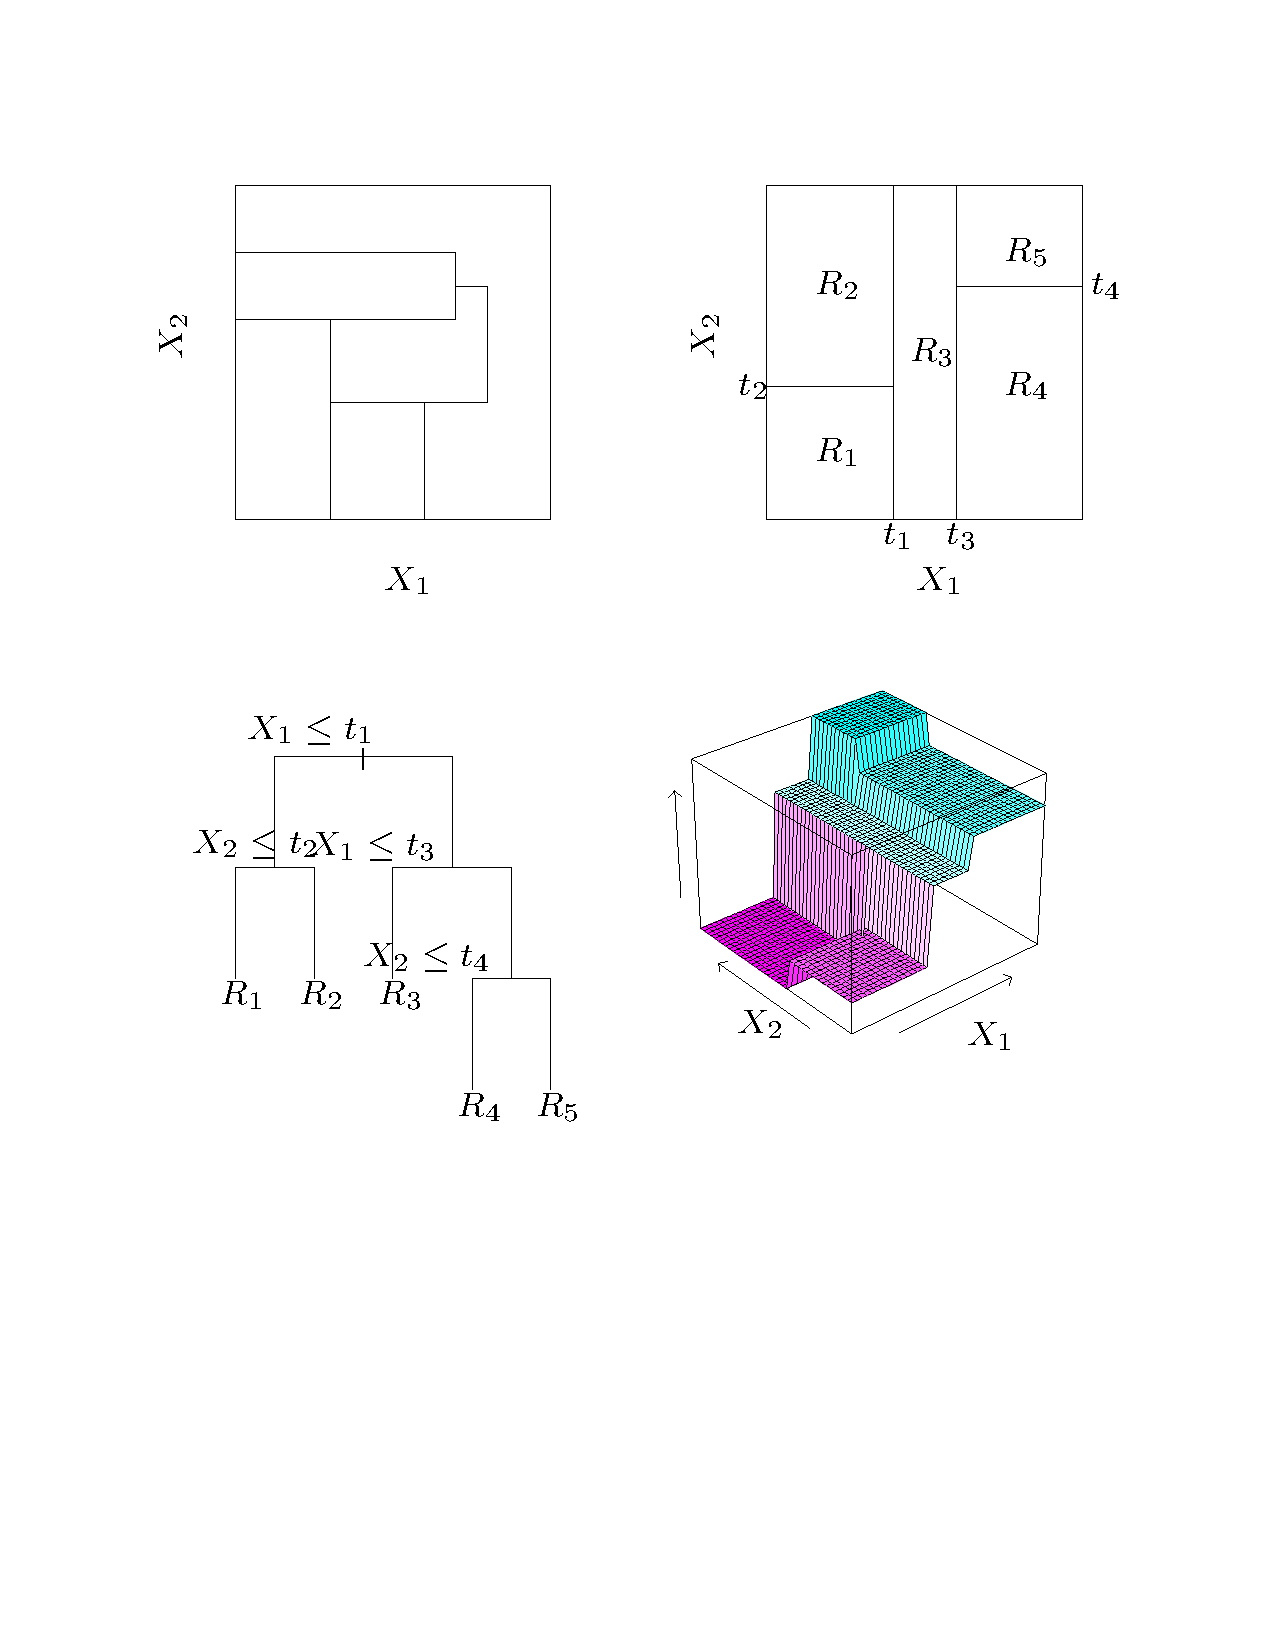
\includegraphics[width=\textwidth]{figures/cart.pdf}
        \end{figure}
\end{columns}
\end{frame}


\begin{frame}{Regression tree fitting}
    \begin{itemize}
        \item For CART, it is clear that each region should just be given by the average of the observations to minimize sum of squares.
        \item Best partition is usually not computationally tractable.
        \item Greedy algorithm: Start with all data, choose splitting variable $X_j$ and split point $s$ such that:
        \begin{equation*}
            \min_{X_j, s} \left[ \sum_{x_i \in R_1(X_j, s)} (y_i - c_1)^2 + \sum_{x_i \in R_2(X_j, s)} (y_i - c_2)^2 \right]
        \end{equation*}
        \item For each $X_j$, splitting point $s$ can be found quickly via scanning of the variables.
        \item This process is repeated for each of the regions to grow the regression tree.
        \item Choice of tree size determines complexity of model - too large a tree results in overfitting, too small results in underfitting.
    \end{itemize}
\end{frame}


\begin{frame}{Cost-Complexity Tree Pruning}
    \begin{itemize}
        \item Generate the tree until a minimum node size is achieved.
        \item Let subtree $T \subset T_0$ be any tree that can be obtained by pruning $T_0$.
        \item Cost-complexity criterion:
        \begin{equation*}
            C_{\alpha}(T) = \sum_{m=1}^{|T|} \sum_{x_i \in R_m} (y_i - \hat{c_m})^2 + \alpha |T|
        \end{equation*}
        \item Find the subtree $T_\alpha$ that minimizes $C_{\alpha}(T)$. $\alpha$ controls complexity. Large $\alpha$ results in smaller tree.
        \item Weakest link pruning: successively collapse each node that produces the smallest increase in $\sum_{x_i \in R_m} (y_i - \hat{c_m})^2$.
    \end{itemize}
\end{frame}


\begin{frame}{Classification Trees}
    \begin{itemize}
        \item Instead of squared error, we need to use alternative \textit{node impurity} measures: 
        \begin{description}
        \item[Misclassification error] $1/N_m \sum_{i \in R_m} I(y_i \neq k(m)) = 1-\hat{p_{mk(m)}}$
        \item[Gini index] $\sum_{k \neq k'} \hat{p_{mk}}\hat{p_{mk'}}$
        \item[Cross-entropy] $-\sum_{k =1}^K \hat{p_{mk}}\log{\hat{p_{mk}}}$
        \end{description}
        \begin{figure}
            \centering
            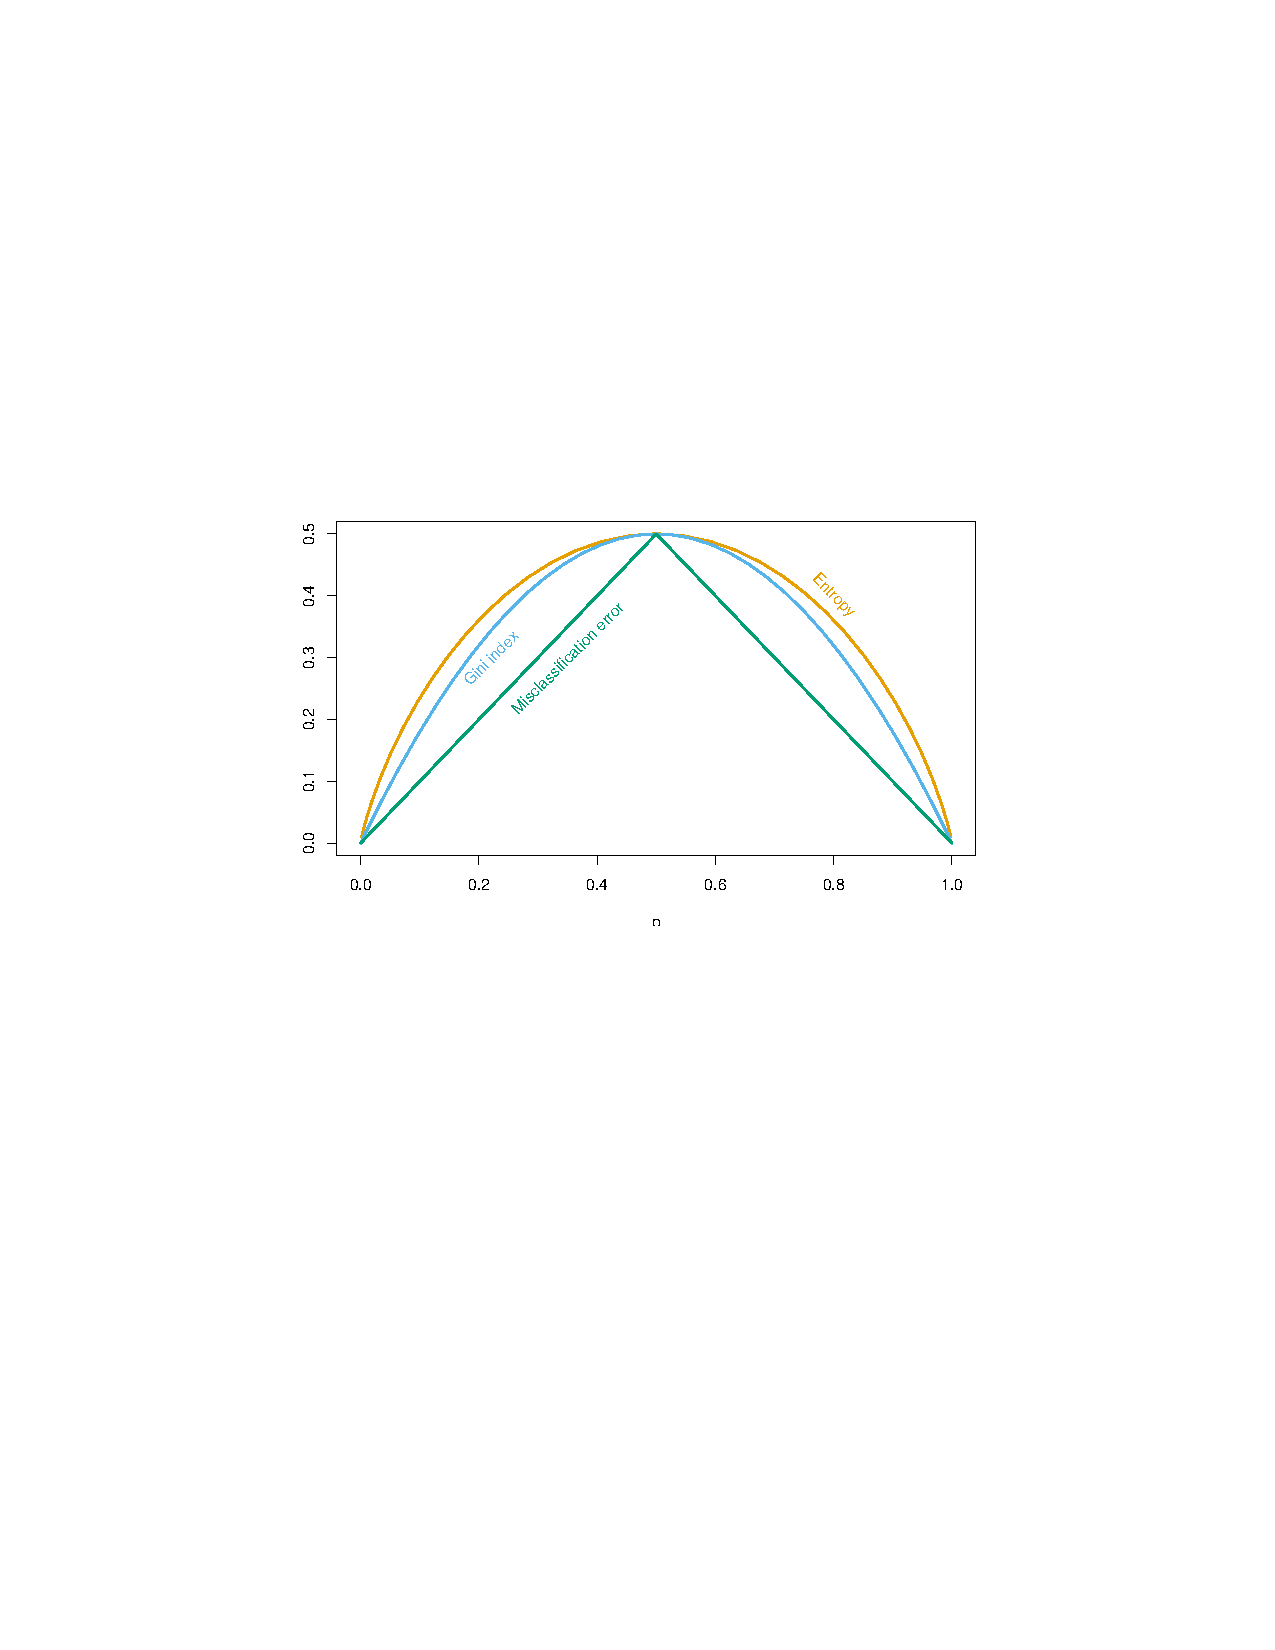
\includegraphics[width=0.6\textwidth]{figures/node-impurity-measures.pdf}
        \end{figure}
    \end{itemize}
\end{frame}


\begin{frame}{Miscellaneous Issues with Trees}
    \begin{itemize}
        \item Trees can be highly interpretable.
        \item Instability: small data changes can lead to very different splits.
        \item Lack of smoothness
        \item For some categorical problems, a misclassification in one category is more serious than another, e.g., it is better to have a false positive for a disease than a false negative. This can be handled by weighting the loss functions appropriately.
    \end{itemize}
\end{frame}


\begin{frame}{Example: Lab 2 revisited}
    \begin{itemize}
        \item We will now play around with the metal/insulator classification problem in Lab 2.
        \item However, we will make a few changes. First, we will not bother with NaN values. Imputing values is ok for many other domains. In materials science, imputing arbitrary values is a recipe for disaster.
        \item Second, we will only select a smaller subset of elemental properties to construct our decision tree with. Namely, AtomicRadius, AtomicWeight, Column, ElectronAffinity, Electronegativity, FirstIonizationEnergy, Row, SecondIonizationEnergy. These properties are available for most elements and we avoid obviously correlated features, e.g., AtomicRadius and AtomicVolume.
    \end{itemize}
\end{frame}


\begin{frame}[fragile]{Decision Tree Regressor and Classifier in scikit-learn}
\begin{minted}{python}
from sklearn.tree import DecisionTreeClassifier, DecisionTreeRegressor
from sklearn.model_selection import train_test_split
from sklearn.tree import export_text

x_train, x_test, y_train, y_test = train_test_split(x, y, test_size=0.1)

decision_tree = DecisionTreeClassifier(criterion="entropy", random_state=0, 
                                       max_depth=5)
decision_tree = decision_tree.fit(x_train, y_train)
train_accuracy = decision_tree.score(x_train, y_train)
test_accuracy = decision_tree.score(x_test, y_test)
r = export_text(decision_tree, feature_names=list(x.columns))
print("Train accuracy = %.3f; test accuracy: %.3f" % (train_accuracy, test_accuracy))
print(r)

decision_tree = DecisionTreeRegressor(criterion="mse", 
                                      random_state=0, max_depth=10)
decision_tree = decision_tree.fit(x_train, y_train)
y_pred = decision_tree.predict(x_test)
\end{minted}
\end{frame}


\begin{frame}{Misclassification rate}
    \begin{figure}
        \centering
        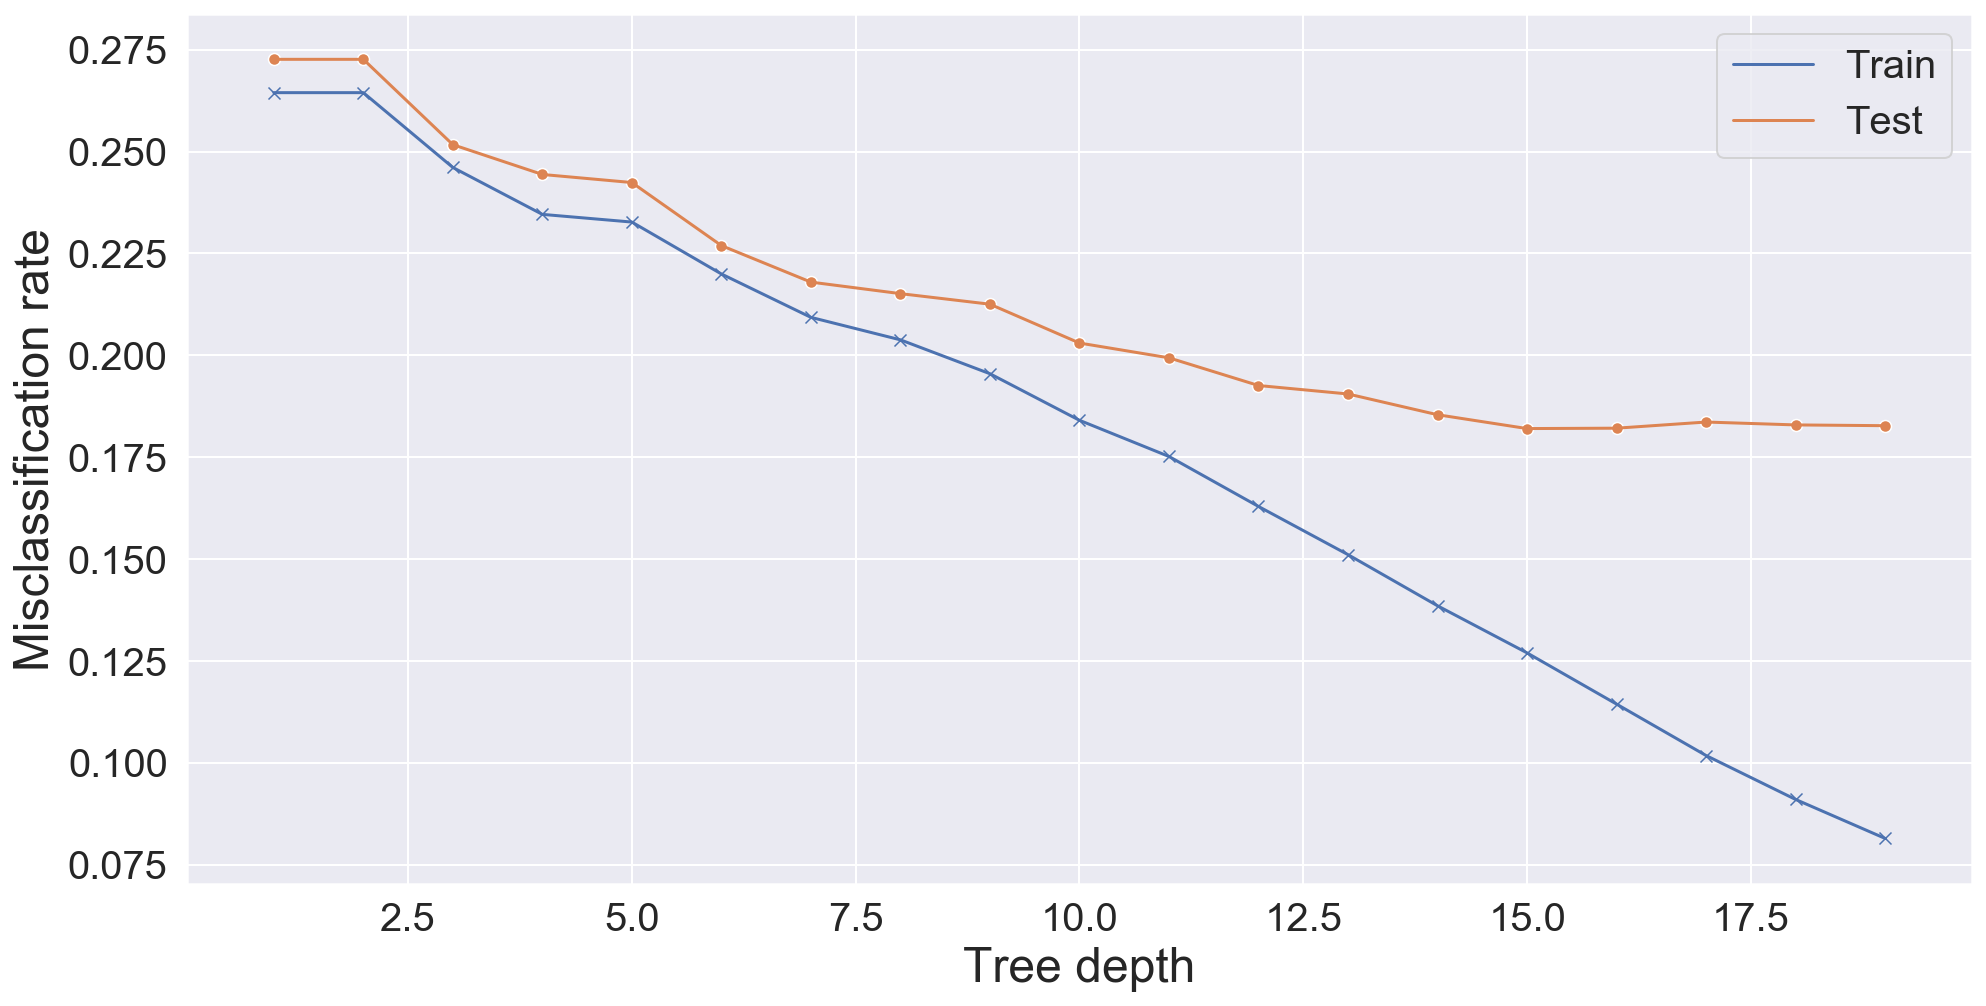
\includegraphics[width=0.8\textwidth]{figures/misclassfication_rate_metal_insulator.png}
    \end{figure}
    \begin{itemize}
        \item Quite clearly, we cannot do much better than a $\sim 82\%$ accuracy (test misclassification rate of about 18\%) with a tree-depth of around 15.
        \item Also, the training and test errors diverge significantly after a depth of around 8, which indicates overfitting.
    \end{itemize}
\end{frame}


\begin{frame}{Interpreting the tree}
    \begin{itemize}
        \item A 8-deep tree is not very easy to read. Here, we will use cost-complexity pruning with a parameter $\alpha = 0.01$ to prune the tree. The resulting tree has an accuracy of around 74\%. Let's see how the decision is being made at the first few levels.
        \begin{figure}
            \centering
            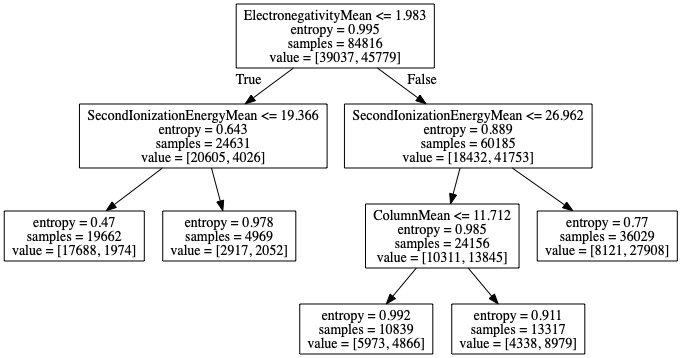
\includegraphics[width=0.8\textwidth]{figures/metal_insulator_tree.png}
        \end{figure}
    \end{itemize}
\end{frame}


\begin{frame}[fragile]{Interpreting the tree, contd.}
\begin{columns}
\column{0.5\textwidth}
\begin{figure}
    \centering
    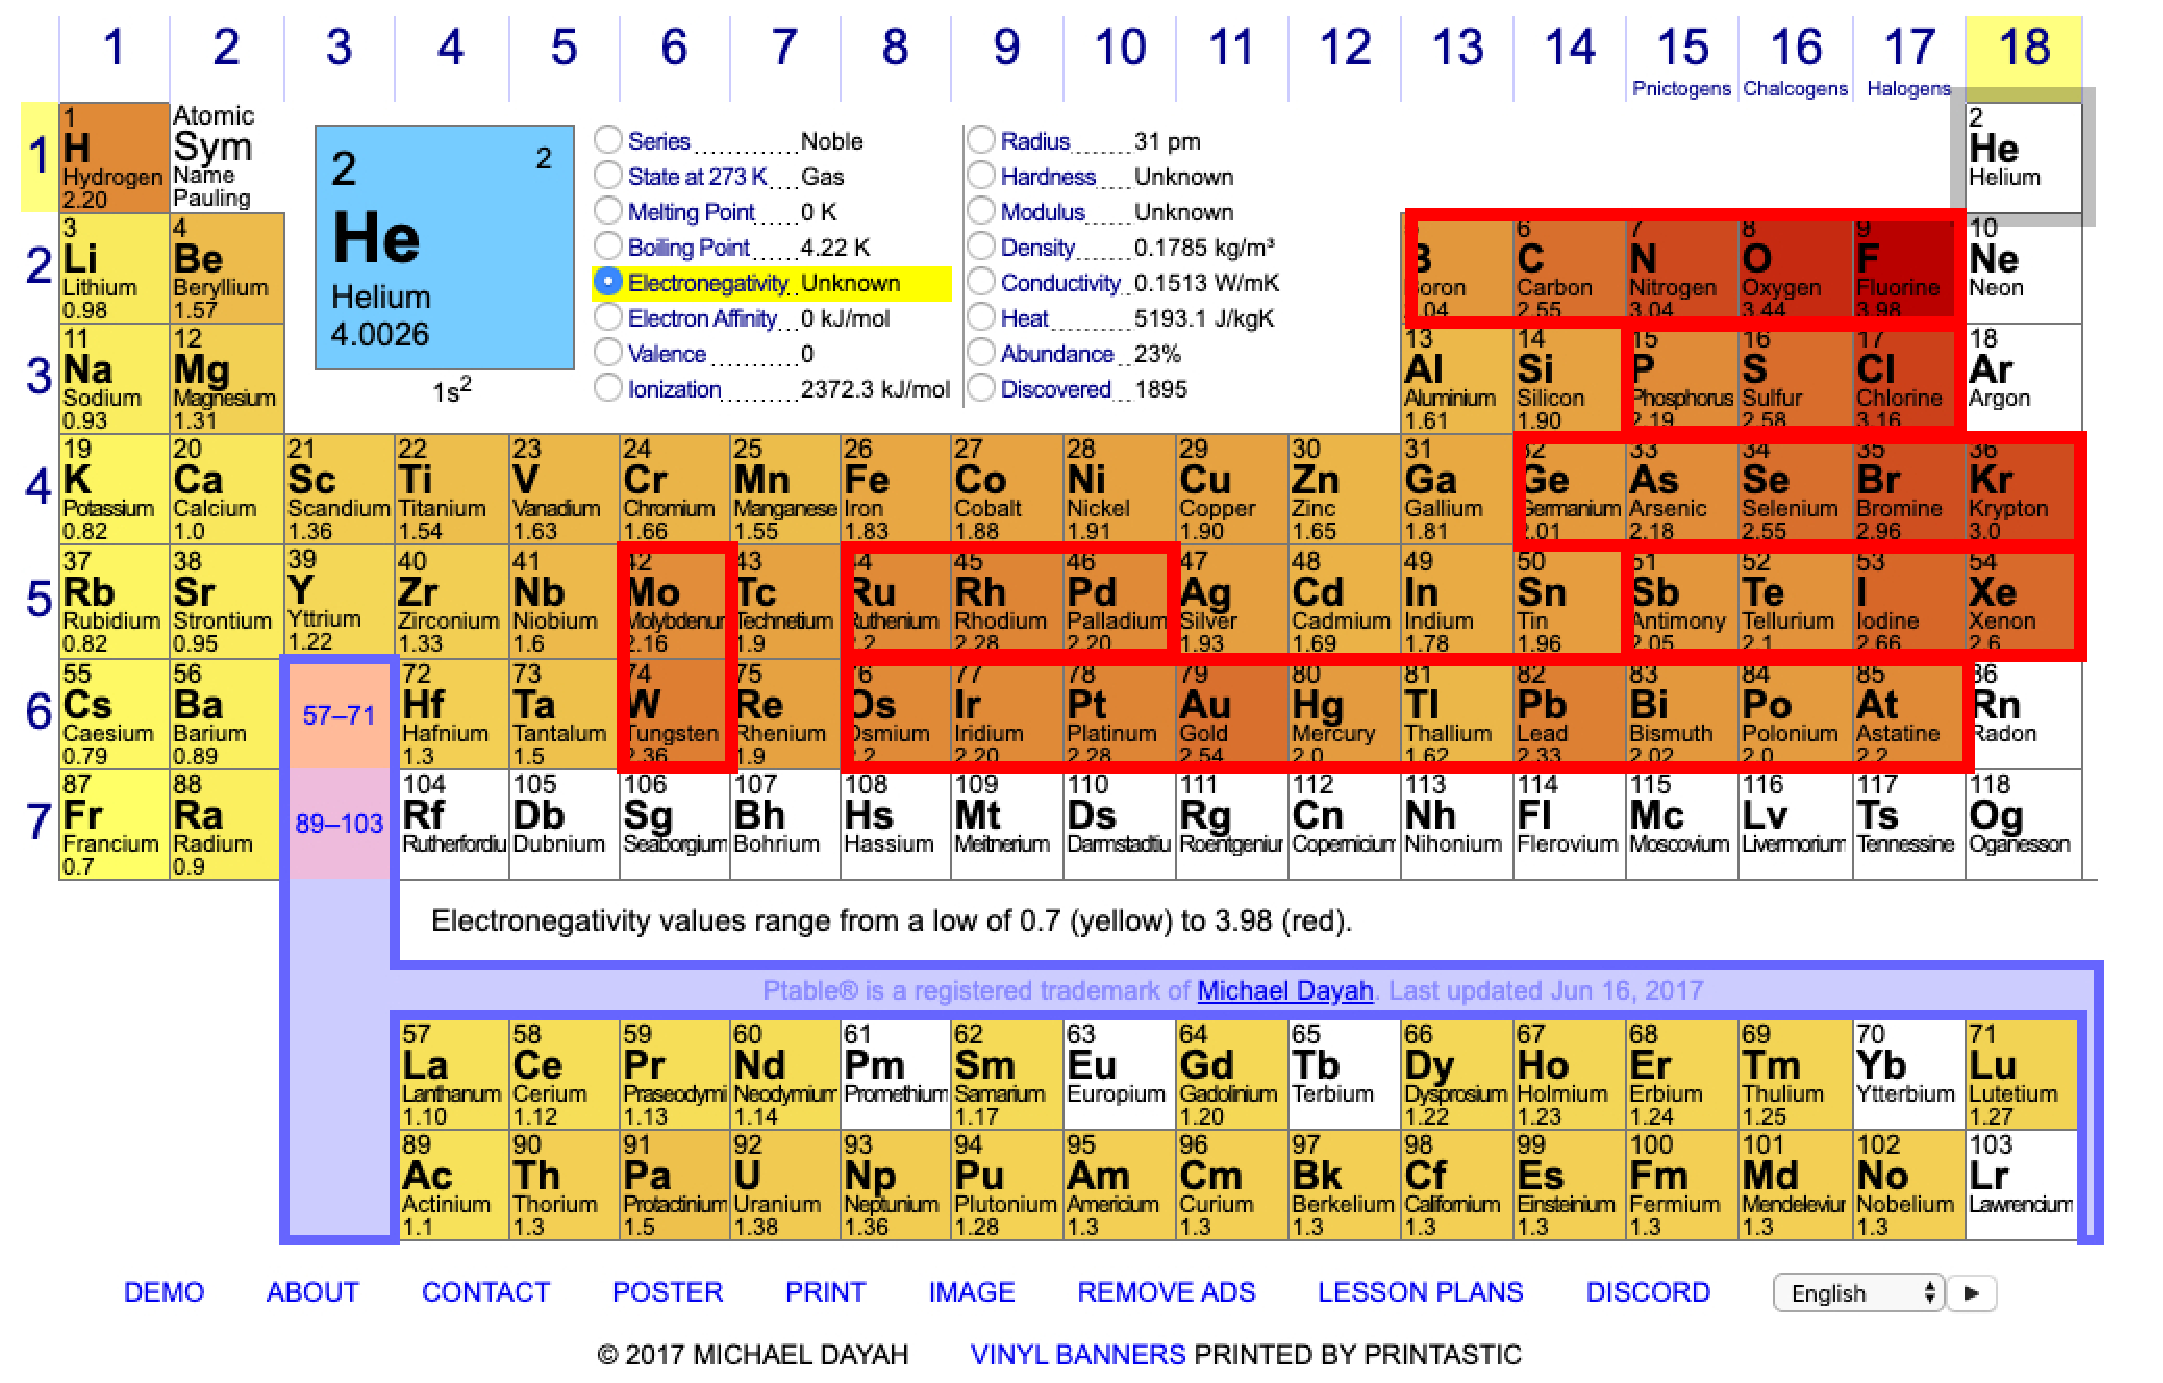
\includegraphics[width=0.8\textwidth]{figures/pt_electronegativity.pdf}
\end{figure}
\scriptsize{
\begin{itemize}
    \item Compounds with mean $\chi \leq 1.92$ are classified as metals.
    \item Compounds with mean $1.92 \leq \chi \leq 2.05$ are classified as metals, unless they contain elements in groups I and II, i.e., ionic compounds.
    \item Compounds with mean $\chi > 2.05$ are insulators unless "AtomicRadiusMean" $>$ 0.97, i.e., metals in group 6, 8, 9, 10, 11.
\end{itemize}}
\column{0.5\textwidth}
\begin{minted}[fontsize=\tiny]{python}
|--- ElectronegativityMean <= 2.05
|   |--- ElectronegativityMean <= 1.92
|   |   |--- ColumnMin <= 2.50
|   |   |   |--- class: 0
|   |   |--- ColumnMin >  2.50
|   |   |   |--- class: 0
|   |--- ElectronegativityMean >  1.92
|   |   |--- ColumnMin <= 2.50
|   |   |   |--- class: 1
|   |   |--- ColumnMin >  2.50
|   |   |   |--- class: 0
|--- ElectronegativityMean >  2.05
|   |--- AtomicRadiusMean <= 0.97
|   |   |--- RowMean <= 2.48
|   |   |   |--- class: 1
|   |   |--- RowMean >  2.48
|   |   |   |--- class: 1
|   |--- AtomicRadiusMean >  0.97
|   |   |--- ColumnMax <= 31.00
|   |   |   |--- class: 0
|   |   |--- ColumnMax >  31.00
|   |   |   |--- class: 1
\end{minted}
\end{columns}
\end{frame}


\begin{frame}
\frametitle{Feature importance}
\begin{columns}
\column{0.5\textwidth}
\begin{itemize}
\item Another way of interpreting trees is using the feature importance.
\item The importance of a feature is the (normalized) total reduction of the criterion brought by that feature.
\end{itemize}
\column{0.5\textwidth}
\begin{figure}
    \centering
    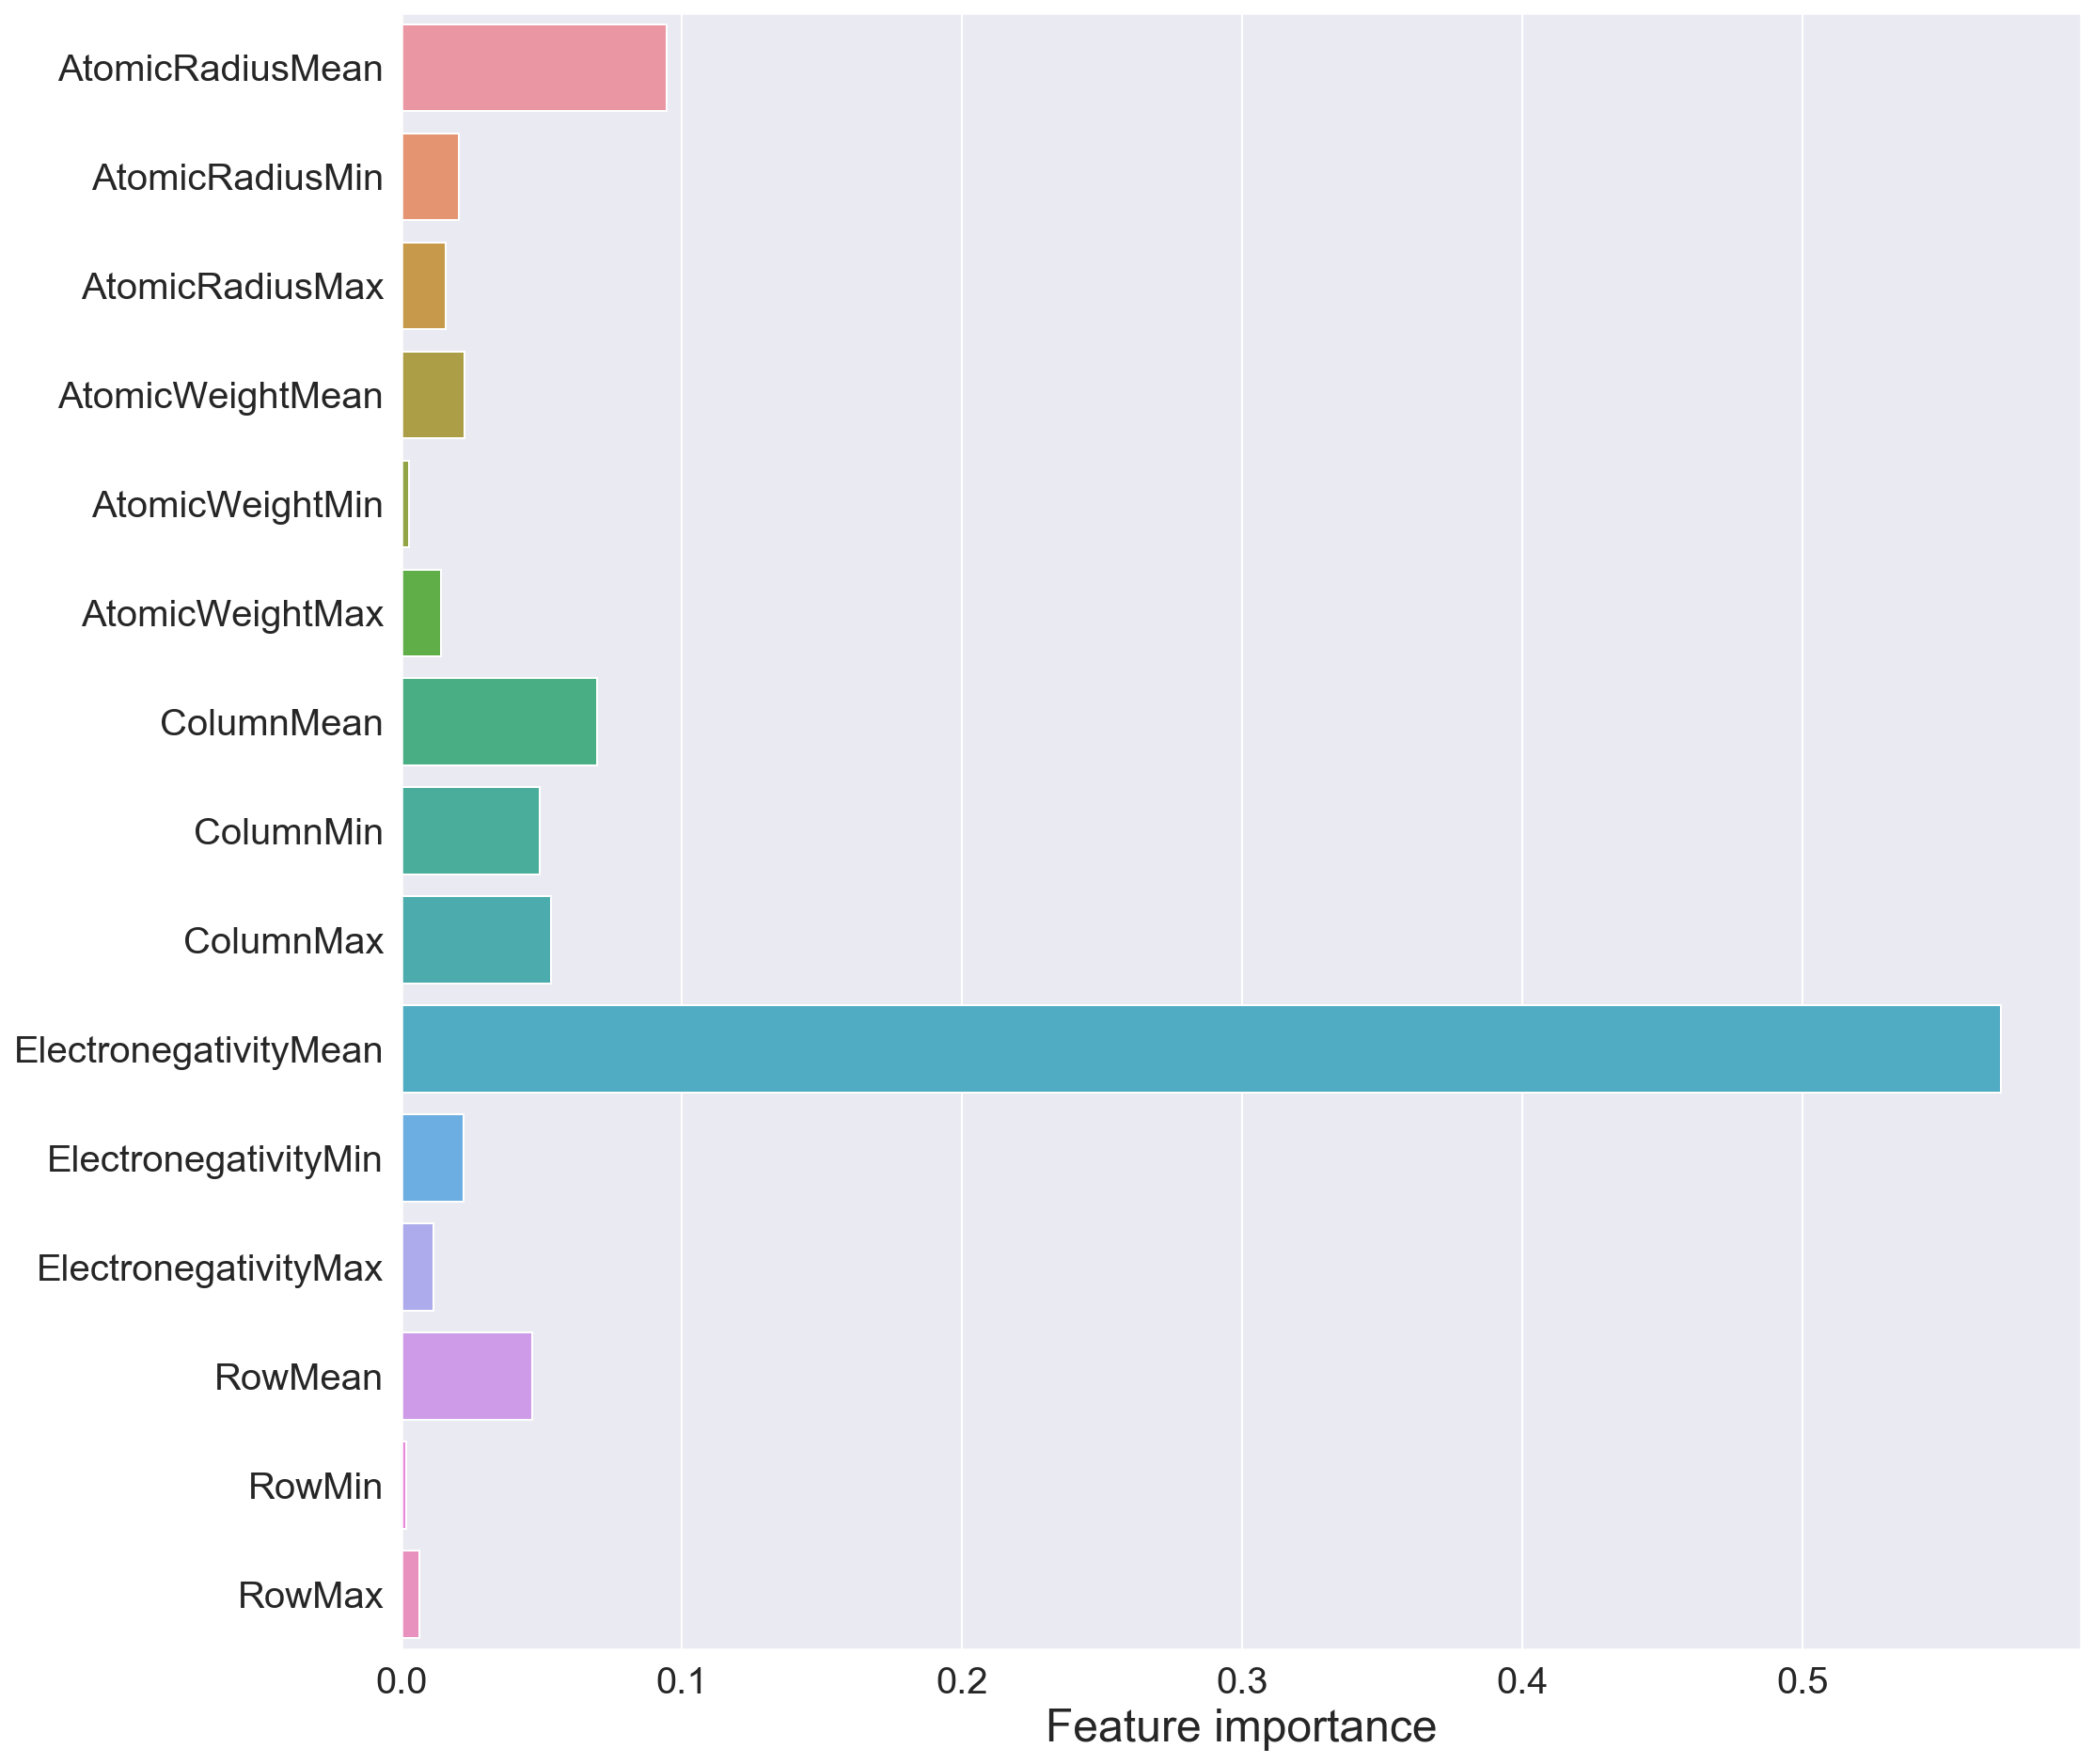
\includegraphics[width=\textwidth]{figures/feature-importance.png}
\end{figure}
\end{columns}
\end{frame}


\begin{frame}{Receiver Operating Characteristic (ROC) Curve}
\begin{columns}
\column{0.5\textwidth}
\begin{eqnarray*}
TPR & = & \frac{TP}{P} = \frac{TP}{TP + FN}\\
FPR & = & \frac{FP}{N} = \frac{FP}{TN + FP}
\end{eqnarray*}
\begin{itemize}
    \item Plot of the TPR (\textit{sensitivity}) vs FPR (1-\textit{selectivity}).
    \item $y=x$ line denotes random guessing (TPR = FPR).
    \item The greater the area under curve (AUC), better the performance.
\end{itemize}
\column{0.5\textwidth}
    \begin{figure}
    \centering
    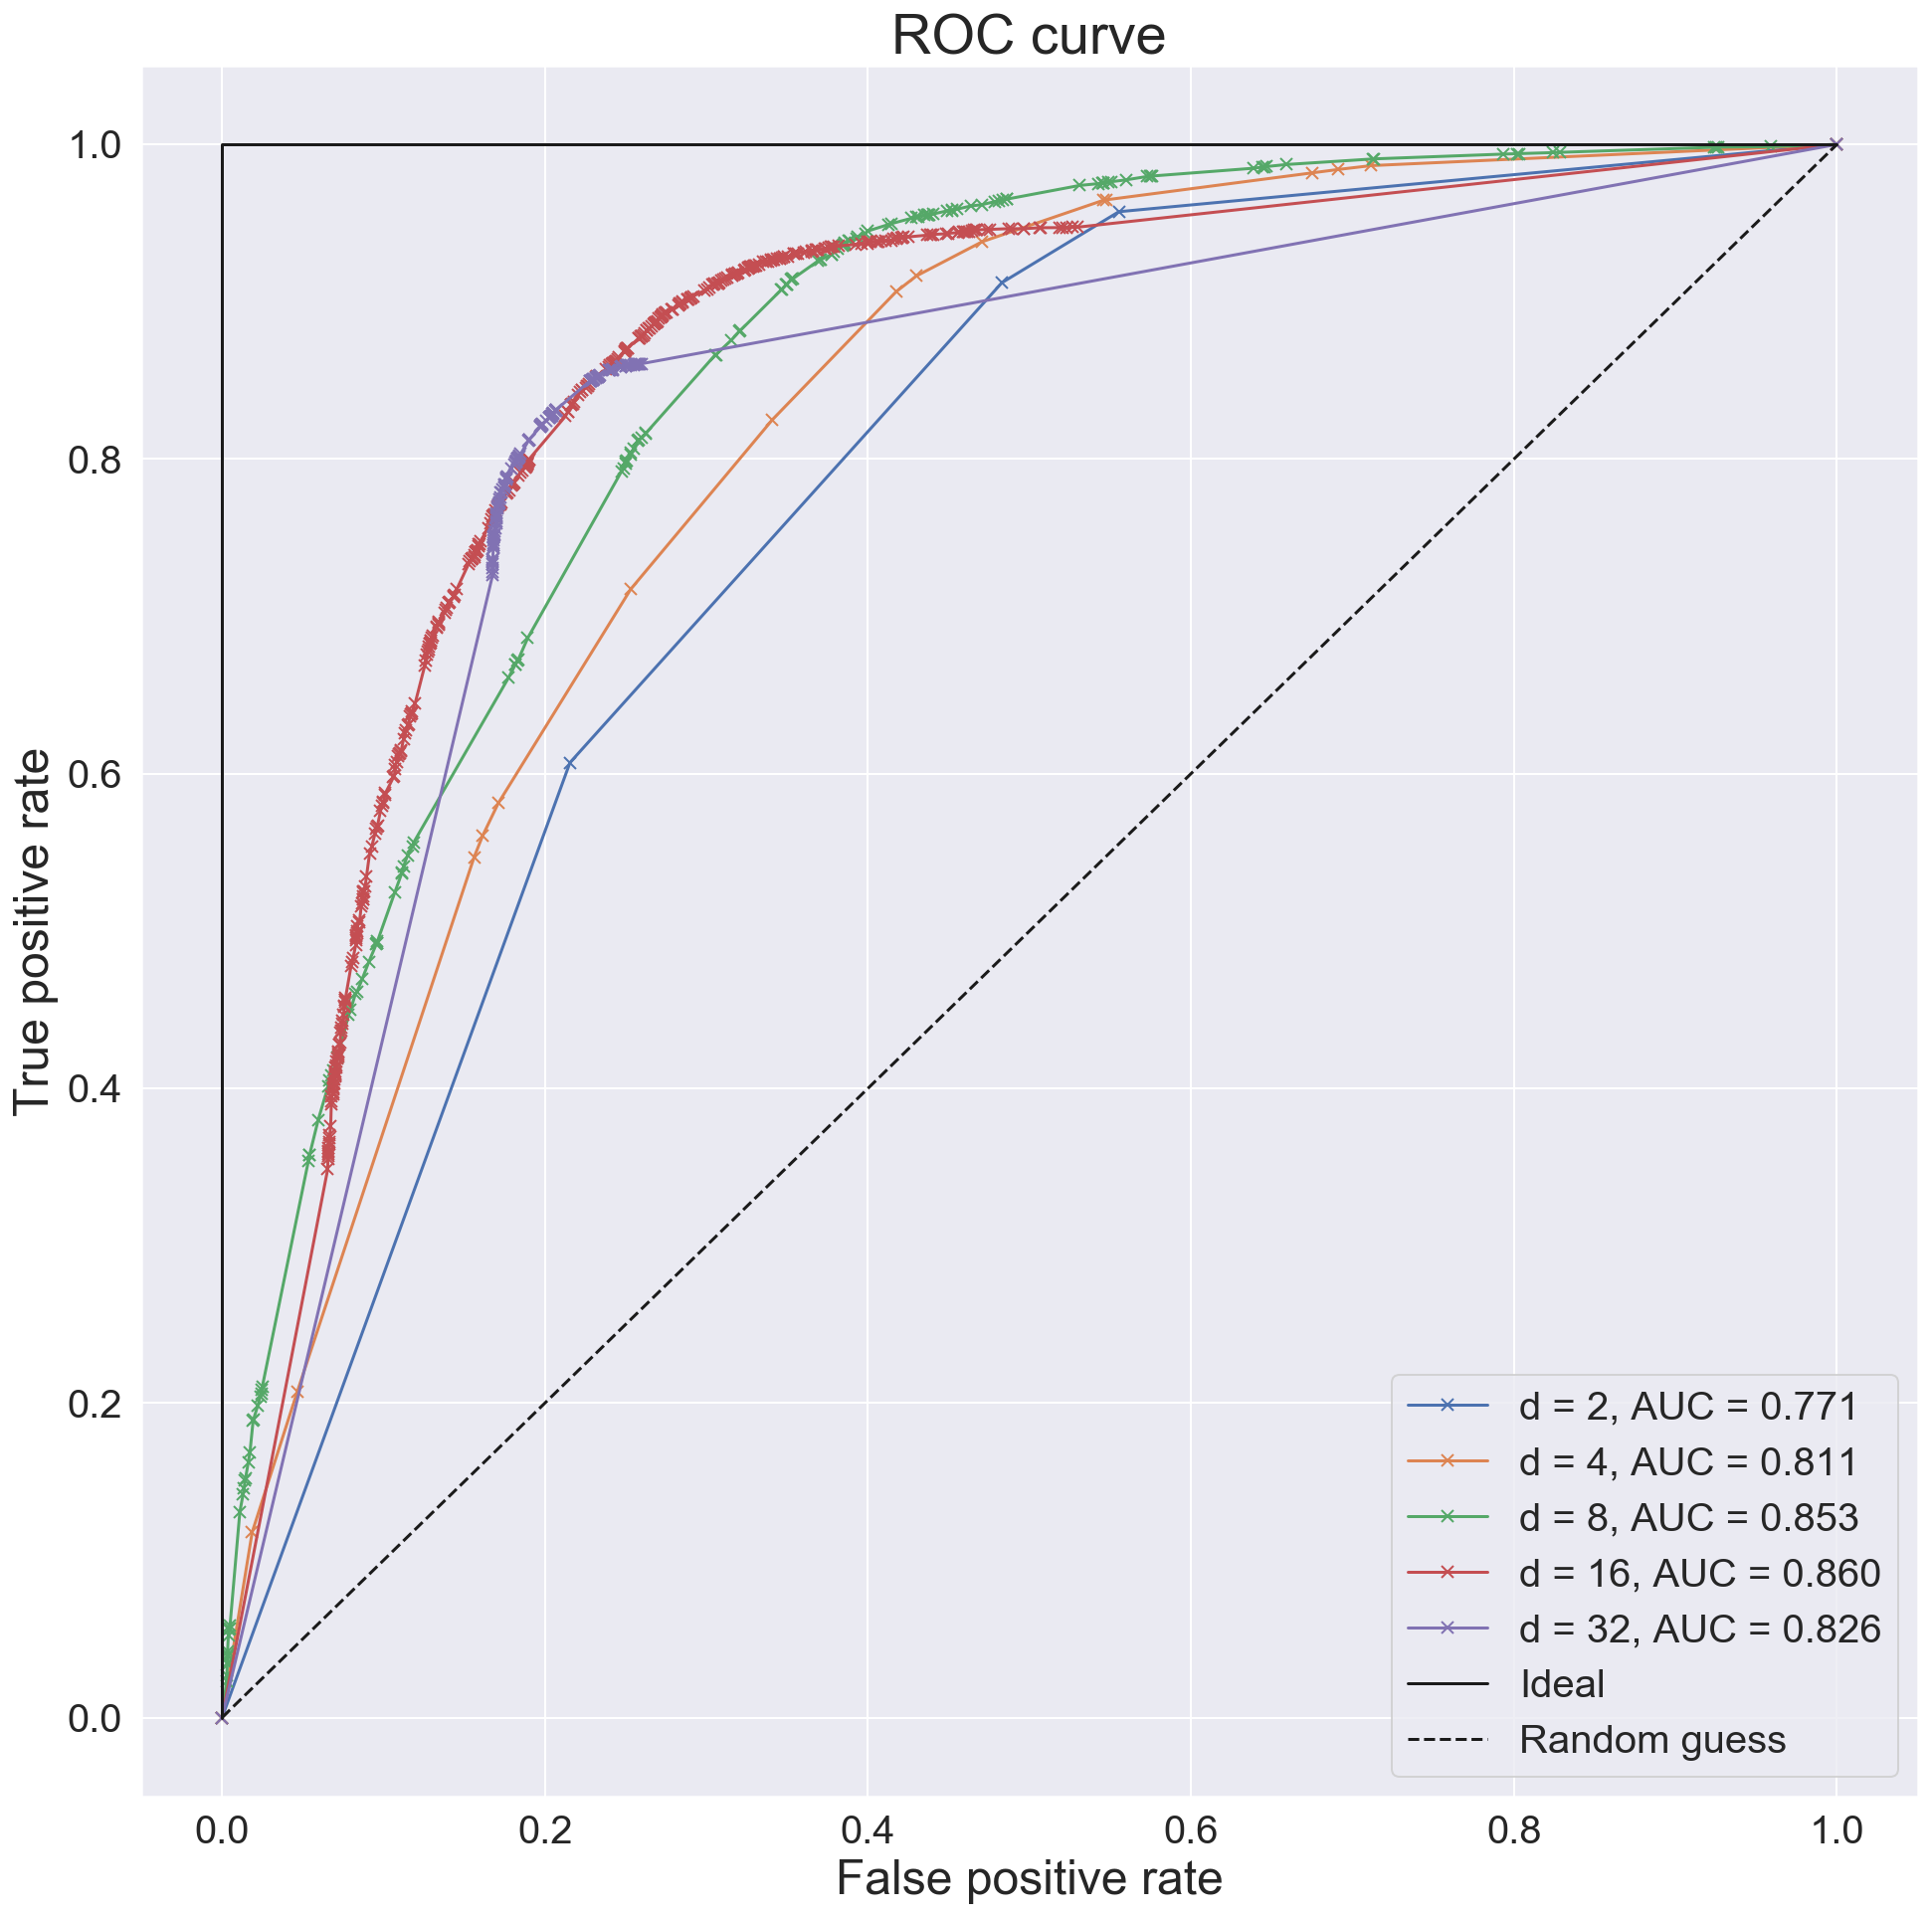
\includegraphics[width=\textwidth]{figures/ROC.png}
    \end{figure}
\end{columns}
\end{frame}


\begin{frame}{Multivariate Adaptive Regression Splines (MARS)}
    \begin{itemize}
        \item Essentially a modification of CART to use step-wise linear regression.
        \item MARS uses piece-wise linear basis functions:
        \begin{equation*}
            (x - t)_+ = \left\{
  \begin{array}{lr}
    x - t &, x > t\\
    0 &, otherwise
  \end{array}
\right.
        \end{equation*}
        \begin{equation*}
            (t - x)_+ = \left\{
  \begin{array}{lr}
    t - x &, x < t\\
    0 &, otherwise
  \end{array}
\right.
        \end{equation*}
        \item Implementation available in the \href{https://contrib.scikit-learn.org/py-earth/index.html}{py-earth} package.
    \end{itemize}
    \begin{figure}
    \centering
    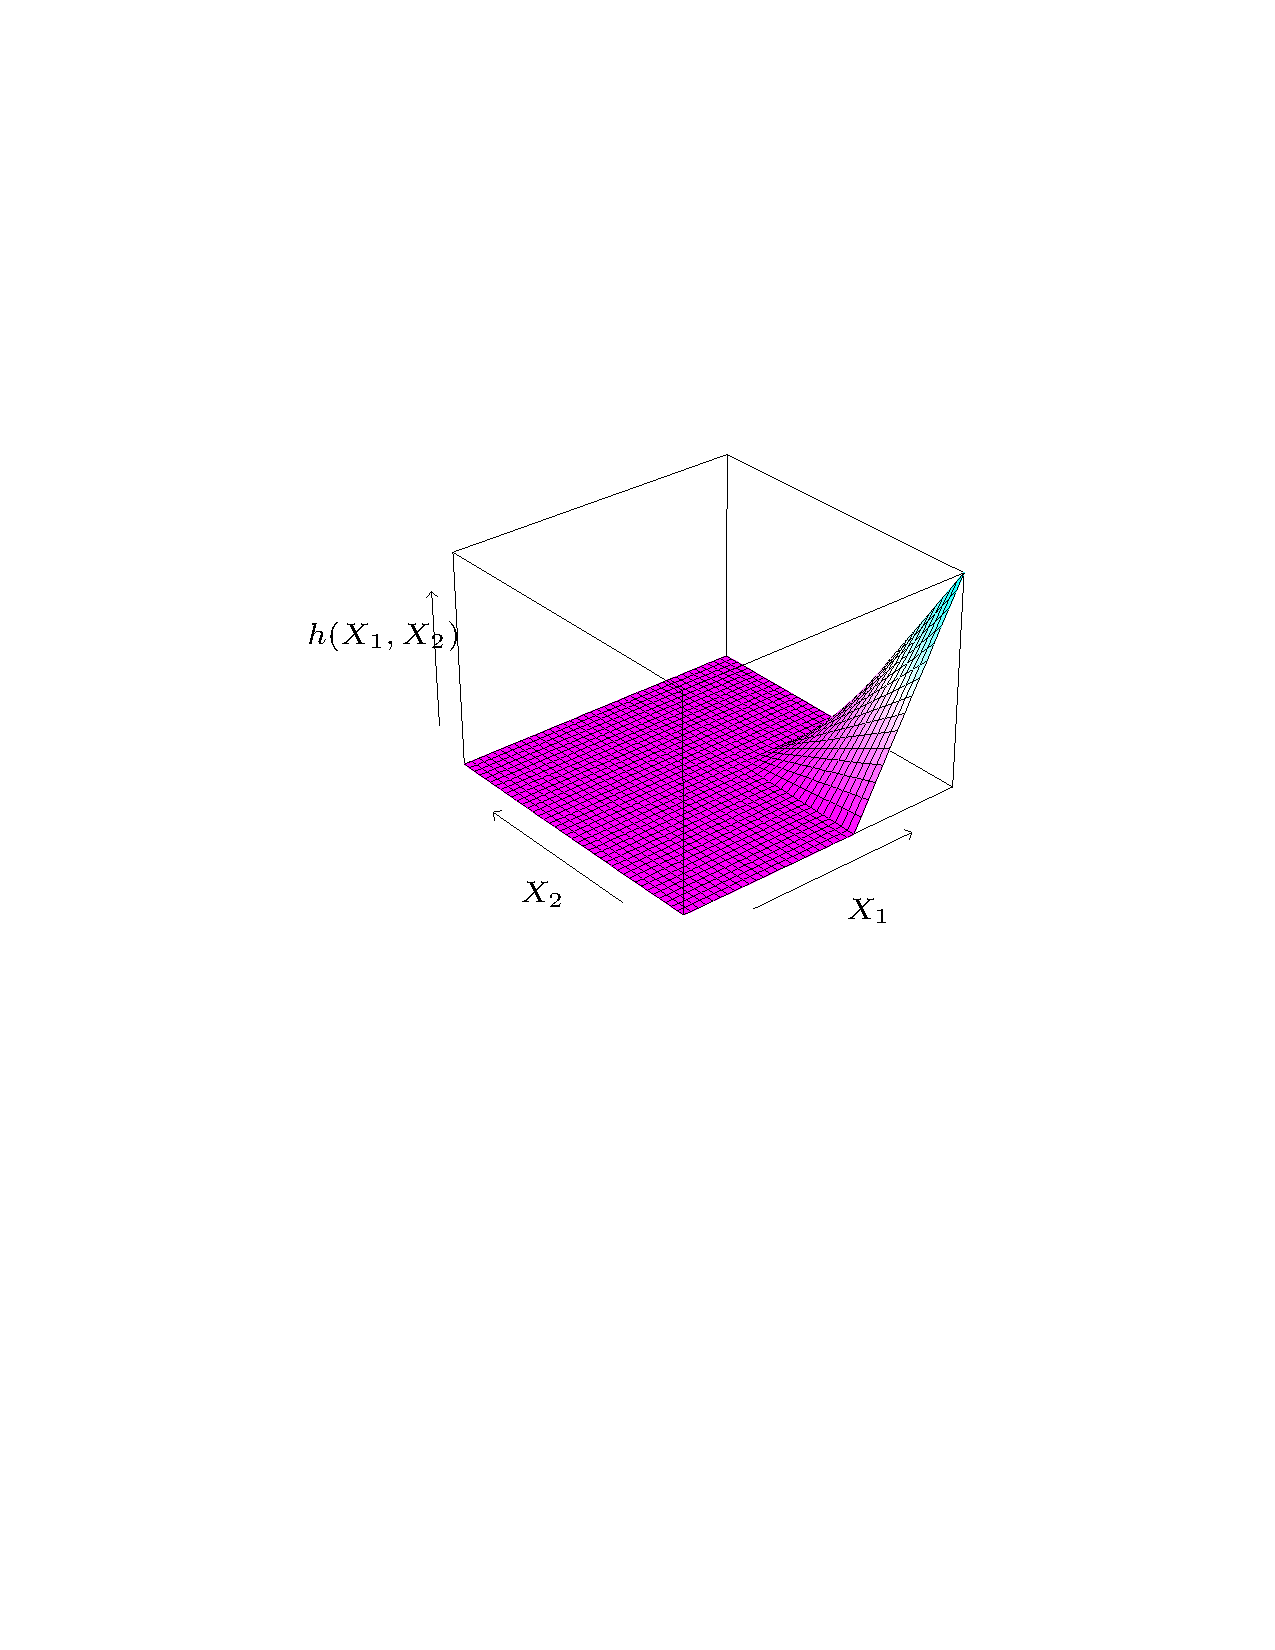
\includegraphics[width=0.4\textwidth]{figures/MARS.pdf}
\end{figure}
\end{frame}


\section{Boosting and Additive Trees}

\begin{frame}{Boosting}
    \begin{itemize}
        \item One of the most successful ML approaches in the past few decades.
        \item Concept: combine many ``weak'' learners in a ``committee''.
        \item Can be used for either classification or regression.
        \item Weak classifier: One whose error rate is slightly better than random guessing.
        \item Apply weak classifier to repeatedly modified versions of data to produce a sequence of weak classifiers.
        \item Predictions from sequence are combined using weighted majority vote:
        \begin{equation*}
            G(x) = sign\left( \sum_{m=1}^M \alpha_mG_m(x)\right)
        \end{equation*}
        \item Weights $\alpha_m$ are computed by boosting algorithm and is the contribution of each weak learner $G_m(x)$.
        \item While $G(x)$ can be any classifier, we will focus here on using decision trees as the base classifier.
    \end{itemize}
\end{frame}


\begin{frame}{AdaBoost.M1 Algorithm (Classification)}
    \begin{enumerate}
        \item Initialize observation weights as $w_i = 1/N$.
        \item For $m=1$ to $M$:
        \begin{enumerate}
            \item Fit classifier $G_m(x)$ to training data using weights $w_i$.
            \item Compute:
            \begin{equation*}
                err_m = \frac{\sum_{i=1}^{N} w_i I(y_i \neq G_m(x_i))}{\sum_{i=1}{N} w_i}
            \end{equation*}
            \item Compute $\alpha_m = \log{\frac{1-err_m}{err_m}}$.
            \item Set $w_i = w_i\exp[\alpha_mI(y_i \neq G_m(x_i))]$, $i = 1, 2, ...N$. Conceptually, increase weights in step $m$ for observations that are misclassified in step $m-1$.
        \end{enumerate}
        \item Output $G(x) = sign\left( \sum_{m=1}^M \alpha_mG_m(x)\right)$
    \end{enumerate}
\end{frame}


\begin{frame}[fragile]{AdaBoost in scikit-learn}
\begin{minted}{python}
from sklearn.ensemble import AdaBoostClassifier

x_train, x_test, y_train, y_test = train_test_split(x, y_class, test_size=0.2)

decision_tree = AdaBoostClassifier(DecisionTreeClassifier(criterion="entropy", random_state=0, max_depth=3), 
                                   n_estimators=20)
decision_tree = decision_tree.fit(x_train, y_train)
train_accuracy = decision_tree.score(x_train, y_train)
test_accuracy = decision_tree.score(x_test, y_test)
\end{minted}
\end{frame}



\begin{frame}{Bibliography}
    \bibliographystyle{unsrt}
    \bibliography{refs}
\end{frame}




\begin{frame}
    \Huge{\centerline{The End}}
\end{frame}

\end{document}

